\chapter{緒論}

% 標題: (近紅外光)任兩點 LED與光電二極體 室內 任兩點 三維相對位置 最佳化組態

\section{前言} %(工業4.0的篇幅)

隨著工業4.0的發展,著重於自動化、互連性,機器、人與環境之間的交互互動愈發頻繁,藉著物聯網(IoT)的能力,各領域對於量測資訊的需求大量增加,其中物聯網所包含的應用領域包含智慧工廠、智慧病房、智慧城市等參考圖\ref{pic:iot}\cite{iot}。

\begin{figure}[ht]
    \centering
    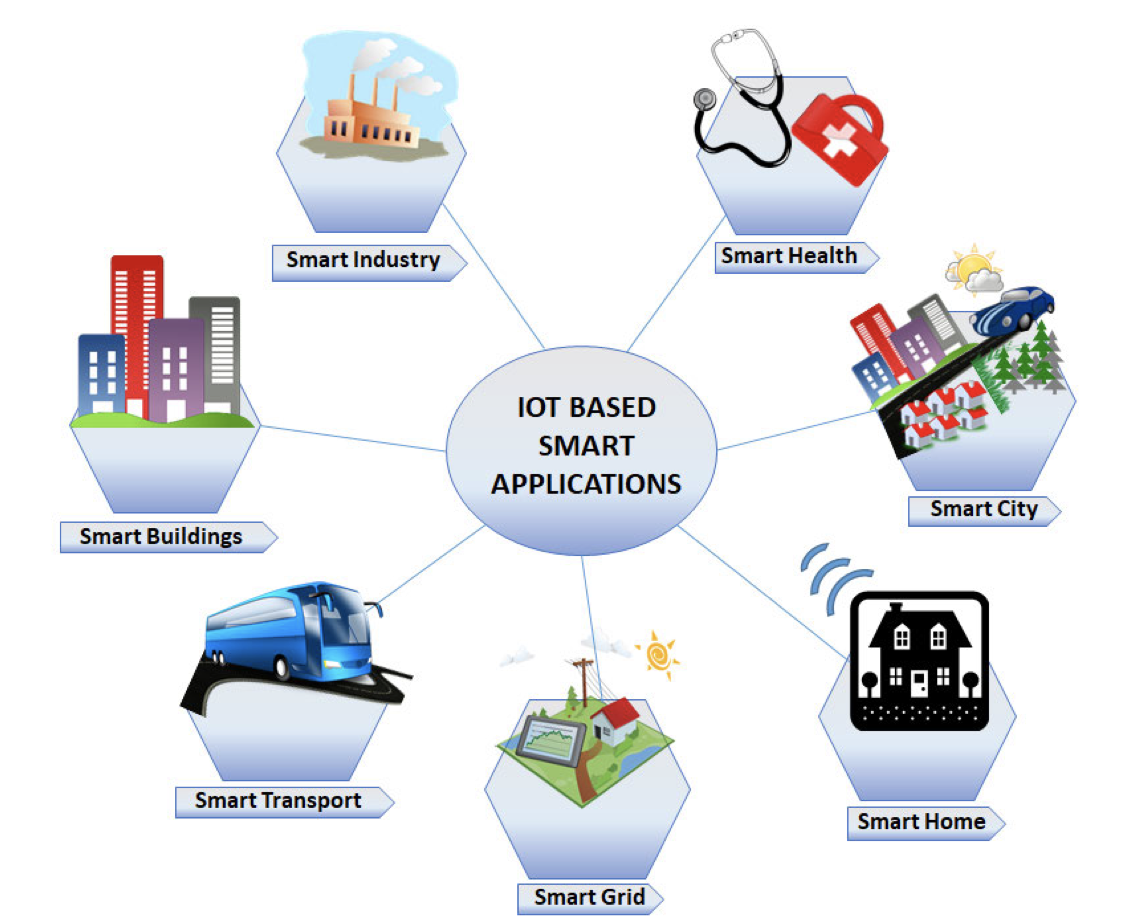
\includegraphics[width=8cm]{ch1pic/iot.png}
    \caption{物聯網應用的領域\cite{iot}}
    \label{pic:iot}
\end{figure}

在萬物互連的背景之下,感測器就像是人類的感官,透過不同種類的探測器量測各式各樣所需的資訊,例如位置、溫度、濕度、電壓、電流、轉速、流速、振動、影像等,各物體之間交換資訊,再透過電腦或是人為操作,下達任務與決策。各項量測資訊之中,相對位置為一重要量測資訊,缺乏位置資訊時,則像是失去地圖的駕駛,或是蒙住眼睛的人們,對於無論是移動、導航、一指令的下達與否,各重決策行為都會難以判斷。除此之外,定位在實務上也充滿挑戰,由於沒有任何一種感測器可以直接量測到相對位置,定位僅能透過多個感測器量測到的距離、角度、影像等資訊,透過校正、運算以獲得定位資訊,並不像是量測距離、溫度等感測器得以直接獲得的物理量一樣簡單。



室外場域中,相對位置需求最常見於載具,例如無人機之間的相互定位,以及自駕車之間的跟隨與溝通;除了載具以外,相對定位的量測在搜救、目標跟隨、監視等情況下都有需求\cite{outdoor_scenario}。現今室外定位主要仰賴全球衛星定位系統(Global Positioning System,以下簡稱GPS)\cite{GPS_important},其原理是利用接收來自三個以上的衛星訊號,透過訊號傳輸時間判斷與各衛星的距離,進而獲得接收者的位置。即使現今的GPS既容易取得又有相較高精度\cite{survey_light2020},然而礙於衛星訊號受建築物體遮蔽的特性,GPS仍然無法在市區、室內等障礙物較多的場域取得較高精度的定位\cite{survey_light2018},

隨著工業4.0的發展,室內應用物聯網技術的場域愈發多樣,例如圖\ref{pic:iot}內提到的智慧工廠、智慧病房、智慧建築等場域,也因此帶動了室內定位的需求。然而,由於室內定位無法使用GPS技術,且室內定位的精度要求大多較室外定位高,因此發展一有效的室內定位方法獲得許多討論與研究關注\cite{survey_indoor2014}。室內定位主要面對的困難與室外不同,室內定位需面對較多的障礙物、牆壁、人員物體的密集度使多重路徑傳輸(Multipath propagation)影響大,也使訊號衰減與散射較為嚴重,以上議題都會增加誤差與難度。眾多文獻中,\cite{survey_light2018}\cite{survey_indoor2014}\cite{survey_indoor2018}\cite{survey_light2020}\cite{survey:indoor_wayfinding}皆提到相較可利用GPS系統的室外定位,室內定位的難度更高,且使用的硬體、演算法百百種,各自有優缺點,至今仍沒有一個領先群雄的解法。因此,我們於於\ref{chp:motivate}章釐清本研究的研究目標情境,再於\ref{chp:intro}章了解室內定位需考量的面向,並以便挑選出最合適的系統。






\section{目標情境}
\label{chp:motivate}
% 前言
我們的主要目標為研究一移動物對另一特定物的相對定位方法,希望能將感測器與訊號發射器包裝成安裝方便的單位,成為可攜式的裝備。使用時,提供一量測單位與一被量測單位,兩者兼具易安裝、易移動的特性,得以靈活的將兩單位各自安裝在量測物與目標物上,在不同場域下進行三維的相對定位量測。

此目標是為了提供一彈性、能夠廣泛應用的設計,以彌補現今定位系統缺少的靈活度。現今大多系統皆是針對特定場域與地點、需大量事先校正與設置,但凡更換環境該系統則失效,難以廣泛應用。

因此,本研究最著重的面向為靈活度以及低演算法複雜度以達到即時應用的可能性;為了使硬體包裝成方便移動安裝的單位,則需選擇硬體體積較小的技術;再來為了能夠廣泛應用,則希望以較低成本的方法施做。

為更具體呈現目標的使用情境,以下舉實例描述:
\begin{description}
    \item[- 智慧工廠] \hfill 
    
    \quad \quad 
    隨著工業4.0與5.0的發展,人機互動以其機器間的互動越加頻繁,且工廠內也會從同品項大量製造,變成變化度高的製程,因此擁有靈活的量測單位實為重要,可以隨時安裝在需定位的人、機械手臂、載具等上面,根據工作不同改變。

    \item[- 智慧病房] \hfill 
    
    \qquad
    隨著輔具、病床智慧化,擁有靈活安裝的定位系統,能夠幫助機器與患者之間的定位,也能夠不受患者移動或是更動醫療器具影響。
    
    \item[- 其他]  \hfill 
    
    \qquad
    智能載具與服務目標的定位、輔助視障者理解目標方向、機場內針對各種載具與行李運送的量測、展場內的偵測引導等。
\end{description}

% 補實例圖








\subsection{室內定位考量的面向}
\label{chp:intro}
% 室內定位的簡介:(範圍對點、點對點、應用情境)




室內定位的方法非常多樣化,本論文參考\cite{survey_indoor2018},將室內定位依照技術(Technology)與方法(Technique)分類:技術所針對的是目標與量測者傳送訊號所使用的硬體種類,常見的技術包含相機、紅外線、可見光定位、無線網路(以下簡稱WiFi)、藍芽、無線射頻辨識(Radio Frequency IDentification,以下簡稱RFID)等不同技術,於\ref{chp:technique}中會更詳盡的介紹。

而方法則是探討不同訊號皆收與處理的方式,從接收訊號資訊的種類可分為訊號強度、時間、與角度;如何利用所接收到的資訊,進一步解出相對位置則於定位演算法分類,常見的包含多點定位(Multilateration)、三角測量(Triangulation)、指紋法(Fingerprinting)、以及利用幾何關係求解的演算法,於\ref{chp:method}中會進一步介紹。


在選擇合適的技術與方法以設計室內定位系統時,需考量許多面向,以下介紹室內定位需考量的因素,以及各面向與不同技術(詳述於\ref{chp:technique})、方法(詳述於\ref{chp:method})的關聯:

\begin{description}
    \item[- 精度]\hfill 
    
    \qquad
    量測精度為量測所得的位置與目標物真實位置之間的歐幾里德距離(Euclidean Distance,以下簡稱歐式距離),多以公尺表示\cite{survey:indoor_wayfinding},普遍精度最高的技術為相機、紅外光\cite{survey_indoor2014},精度大多會在公分量級上下;相較精度較低的則為WiFi與藍芽,精度常會在公尺量級上下\cite{survey_indoor2014}。然而為了達到高精度,需要與大多面向做取捨\cite{survey:indoor_wayfinding},例如欲達到較高的量測範圍、低成本、高靈活度等,都需要捨棄部分精度,難以同時兼顧。
    
    \item[- 量測範圍] \hfill  
    
    \qquad
    相機、紅外光、可見光量測範圍大多會限制在五米內,超出此範圍後定位精度會快速下降;而WiFi、藍芽、RFID等覆蓋範圍則較廣,能夠達到十米以上的定位\cite{survey_indoor2014}。
    
    \item[- 成本] \hfill 
    
    \qquad
    系統成本包含硬體設備成本與系統能耗等,成本與使用的技術種類關係較大,硬體成本屬於中高價位的有相機、紅外線、RFID,而WiFi、藍芽、可見光定位則屬於建設成本較低的選項;能耗的部分則每篇論文皆有不同的看法,如\cite{survey:radio}中認為WiFi為低能耗相較\cite{survey:indoor_wayfinding}認為其為高能耗,各篇論文中並沒有共識。
    
    \item[- 靈活度] \hfill 
    
    \qquad
    靈活度意指:是否能夠靈活的安裝以及使用,而所需的校正時間與系統設置難度都與方法較為相關。如指紋法需先蒐集大量數據,再與數據庫中的資料做交叉比對,此方法便需要花大量時間事先校正,並不能適應環境的改變,但凡環境與系統異動則原數據庫失效,大大限制了靈活度。且若需建立多個錨點(Anchor),也就是在環境中的多個位置放置接收器或是發射器,利用多個錨點的訊號來進行定位分析,此種類型的系統一樣需事先對環境設置與定位,呈現「環境對單點」的定位,系統架設複雜度高。此種類型能夠透過提高錨點的數量來提升精度與量測範圍,眾多技術中,訊號精度較低的技術如WiFi、藍芽、RFID較侷限在這種大規模的系統,靈活度低。


    
    \item[- 是否定位可視範圍外] \hfill 
    
    \qquad
    非可視範圍(Non-Line-of-Sight,以下簡稱NLoS)的定位,會擴大量測範圍,即可不受到環境障礙物的影響,即便是格著牆壁也可以進行定位。然而此舉也同時會造成訊號來源混亂,無法分辨此訊號強度為LoS傳遞而來的,還是穿透何種障礙物之後造成衰減的訊號,進而犧牲精度。而能夠穿透障礙物的多屬於使用低頻率電磁波的硬體技術,如WiFi、藍芽、RFID,此特性也反應較低的精度上。


    \item[- 即時應用] \hfill 
    
    \qquad
    需進行即時應用的情境下,量測數據處理速度需夠快,以避免訊號延遲,因此經常犧牲訊號處理的複雜度及其附加的精度,或是提高成本增加硬體運算能力。訊號處理複雜度高最容易聯想到的便是相機,為了進行視覺辨識的高運算,該類型的系統多配備較好的演算單位\cite{survey_light2020};除此之外,主要影響因素則是該系統的演算法速度,各項技術與方法皆有演算法快與慢的方法,如何設計便是精度、功能與運算速度之間的取捨。
    
    \item[- 目標物是否為特定物] \hfill 
    
    \qquad
    定位技術大多指目標物為特定某物體的情況,因此系統需有分辨訊號發送者的能力,例如WiFi、藍芽、RFID都具有傳送訊息的能力且發展成熟\cite{survey:indoor_wayfinding},可見光與紅外線則是利用近年來發展的光通訊方法進行訊號傳輸,而相機則是利用視覺辨識判斷目標物;反之,超聲波與光達僅有分辨訊號的有無,難以進行目標物辨識,因此大多應用在判斷障礙物存在與否的情境,較少在定位系統上出現。
    
    \item[- 場域限制]\hfill 
    
    \qquad
    特別需要注意的是機場與醫院,這兩種場域有可能會限制無線電波的使用\cite{case:vlc_mobile},因此使用無線電波段的技術如WiFi、藍芽、RFID則需特別注意。
\end{description}

礙於如此多的特性與面向,一個面面俱到的方案是不存在的。因此在設計系統時,了解不同做法的優缺點,並了解系統目標情境與需求,進而對不同面向做出取捨,是完成有效室內定位系統的關鍵之一\cite{survey_indoor2018}。












%[看最後能不能凹到一開始發想是在醫療器具上,結合實驗室研究,這樣可見光就變更合理了]

\section{研究目的}
\label{chp:purpose}
雖然室內定位這個領域已經有許多文獻探討,然而針對此靈活度高、成本低、應用度廣泛的方法,仍沒有一個合適的方案。因此以這幾個面向為重點,於\ref{chp:method}與\ref{chp:technique}中逐漸聚焦於發光二極體(Light Emitting Diode,以下簡稱LED)與光電二極體(Photodiode,以下簡稱PD)的近紅外光定位。針對此種技術與方法,設計一不限制應用場域,且目標物能夠自由移動的定位演算法,主要改善現今定位系統的侷限度,並將LED與PD定位系統中經常被忽略的硬體參數以及組態完整加入考慮。除了提出演算法外,針對不同使用情境進行最佳化,藉由挑選合適的硬體參數與組態,以提升系統定位精度與量測範圍。

% 目標:低成本、不受環境影響、可分辨目標物、快速



\begin{itemize} 
    \item{聚焦於光波段定位}:為了發展一靈活度高,能夠套用在不同場域與情境的室內定位方法,由不同方法與技術所著重的面向切入,將研究聚焦在光波段定位上。
    \item{完整模擬}:光波段定位的領域中,朗博次方常被忽略,並不符合實際硬體挑選的狀況,因此本研究將其納入考量。
    \item{提出靈活的演算法}:光波段定位的領域中,為了降低系統的複雜度,經常限制使用情境,例如限制目標物與觀察者需為平行,因此本論文提出一不限制情境的三維定位演算法,並以模擬分析誤差。
    \item{針對情境最佳化}:將提出的演算法套用在不同的使用情境上,發展一套完整流程,針對其進行組態與硬體參數的最佳化。
\end{itemize}

% 補想像圖








\section{論文架構}
本研究分為六個章節,論文架構如下:

\begin{description}
    \item[第一章] 緒論
    
    介紹研究主題,並描述本研究欲解決的問題與研究目的。
    
    \item[第二章] 文獻回顧
    
    介紹室內定位的不同技術與方法,並聚焦在利用LED與PD的光定位方法,提出此技術現今研究所不足面向。
    
    \item[第三章] LED與PD定位演算法
    
    詳細說明本研究利用LED與PD的相對定位演算法。

    \item[第四章] 誤差分析
    
    將第三章所提出的演算法進行誤差分析。
    
    \item[第五章] 最佳化
    
    建立針對組態與硬體參數的最機化問題,並提出一流程以針對不同量測情境與工況進行最佳化。
    
    \item[第六章] 案例
    
    針對不同情境進行最佳化,提出最佳解並探討成效。
    
    \item[第七章] 結論
    
    整理本研究之結果討論,並敘述後續研究之方向。
    
    \end{description}







    了解位置資訊,為機器與人類進行判斷與決策的基礎。反之,若能掌握空間中某特定物與自己的相對位置資訊,則可幫助新型載具、機械手臂與人類進行決策與執行任務,例如載具了解其他載具的位置、飛行器與遙控計之間的定位、智能載具與照護目標物的互動、機械手臂與夾取目標物的定位等。


    綜上所述,獲取兩物之間的相對位置資訊,有其必要性。